% Chapter: 02_early_cnn_mechinterp
% Included from lectures/main.tex

\section{Early MechInterp on CNNs}

\begin{frame}{Early MechInterp on Convolutional Neural Networks}
\begin{center}
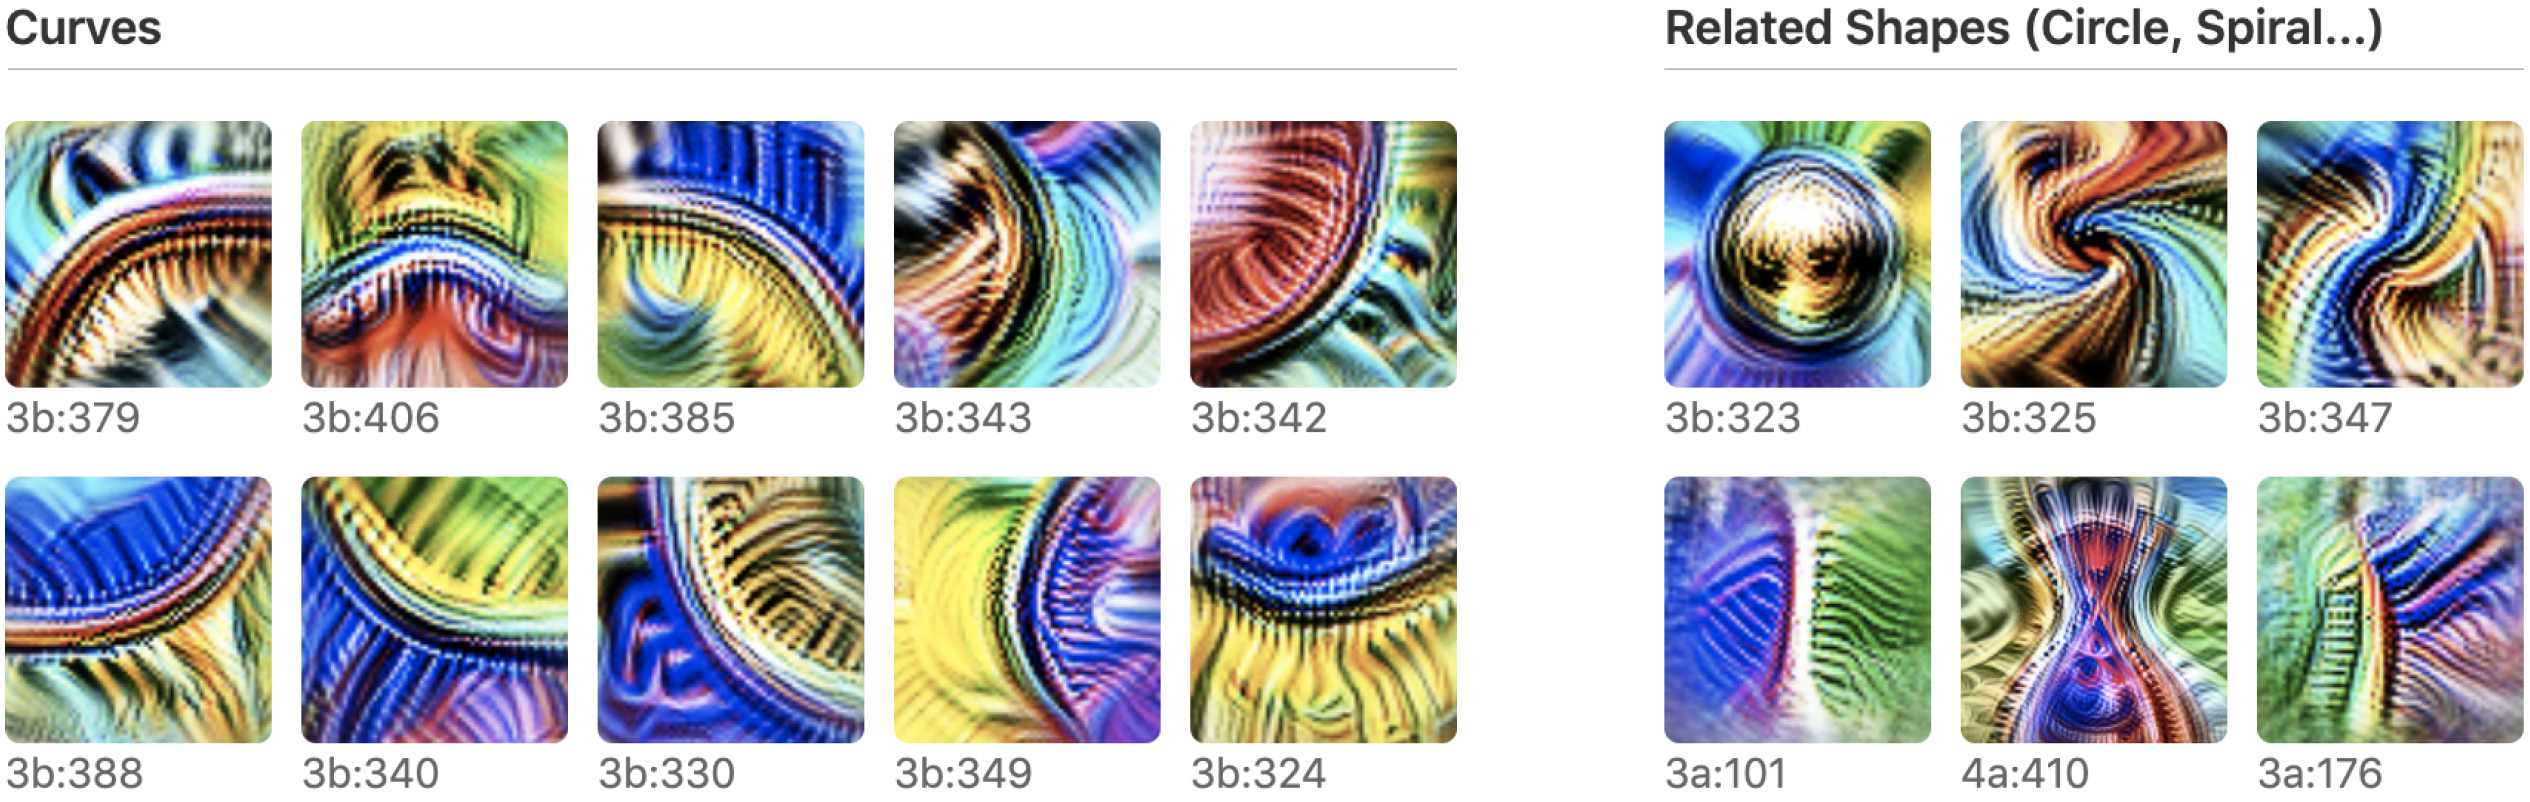
\includegraphics[width=0.8\textwidth]{figures/curves_overview.png}
\end{center}

\note{
\begin{itemize}
\item Most early MechInterp work was done on visual neural networks, typically CNNs
\item Multiple reasons for this
\end{itemize}
}
\end{frame}

\begin{frame}{Why CNNs?}
\begin{itemize}
\item Many early impressive neural networks were visual (e.g.\ AlexNet)
\item CNN channels are a preferred basis, so candidate features are architecturally clear
\item Lots of universality in vision CNNs compared to LLMs
\item Feature visualization works well in vision models
\end{itemize}

\note{
\begin{itemize}
\item Many early impressive neural networks were visual neural networks (e.g.\ AlexNet)
\item MechInterp is easier with convolutional networks: the different channels of a convolutional layer are a preferred basis, which makes the directions that might be features architecturally clear
\item There is a lot of universality in vision CNNs, compared to transformer-based LLMs
\item As we will see, feature visualization works pretty well in vision models
\end{itemize}
}
\end{frame}

\begin{frame}{}
\begin{center}
\Large What would convince you a CNN channel has the function of ``detecting a curve?''
\end{center}

\note{
\begin{itemize}
\item Discussion: what evidence would we demand for that claim?
\end{itemize}
}
\end{frame}

\begin{frame}{Argument 1: Feature Visualization \cite{olah2020}}
\begin{columns}[c]
\begin{column}{0.35\textwidth}
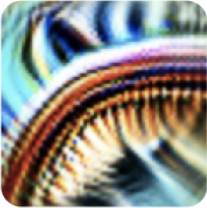
\includegraphics[width=\textwidth]{figures/curve_detector_feature_visualization.png}
\end{column}
\begin{column}{0.6\textwidth}
Optimizing the input to maximally activate curve detectors reliably produces curves.
This establishes a causal link.
\end{column}
\end{columns}

\note{
\begin{itemize}
\item Optimizing the input to cause curve detectors to fire reliably produces curves
\item This establishes a causal link, since everything in the resulting image was added to cause the neuron to fire more
\end{itemize}
}
\end{frame}

\begin{frame}{Argument 2: Dataset Examples \cite{olah2020}}
\begin{columns}[c]
\begin{column}{0.4\textwidth}
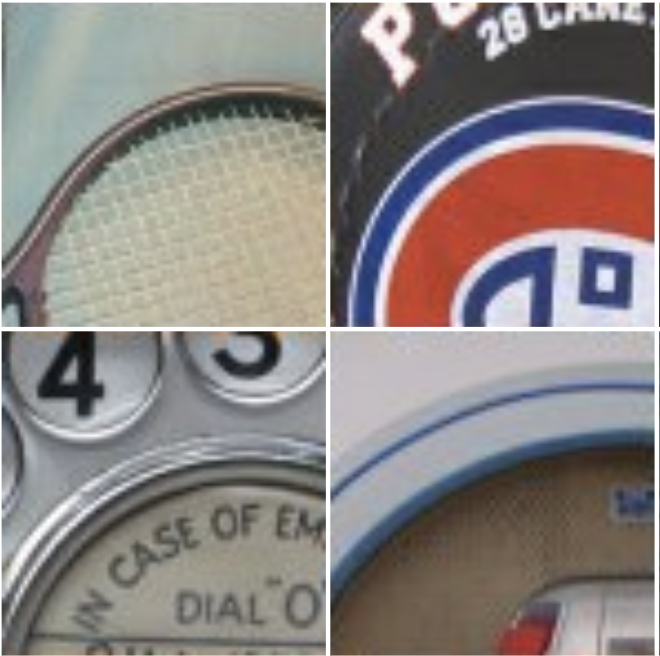
\includegraphics[width=\textwidth]{figures/curve_detector_dataset_examples.png}
\end{column}
\begin{column}{0.55\textwidth}
ImageNet images that strongly activate these neurons reliably contain curves in the expected orientation.
\end{column}
\end{columns}

\note{
\begin{itemize}
\item The ImageNet images that cause these neurons to strongly fire are reliably curves in the expected orientation
\item Images that cause moderate firing are generally less perfect curves or curves off orientation
\end{itemize}
}
\end{frame}

\begin{frame}{Argument 3: Synthetic Examples \cite{olah2020}}
\begin{columns}[c]
\begin{column}{0.4\textwidth}
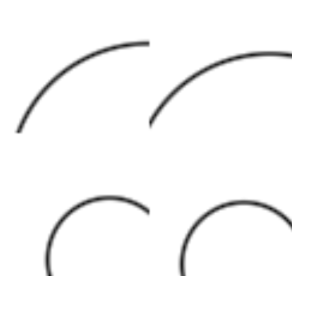
\includegraphics[width=\textwidth]{figures/curve_detector_synthetic_tuning.png}
\end{column}
\begin{column}{0.55\textwidth}
Curve detectors respond as expected to synthetic curves with varying orientations and curvatures.
They do not fire for straight lines or sharp corners.
\end{column}
\end{columns}

\note{
\begin{itemize}
\item Curve detectors respond as expected to a range of synthetic curve images created with varying orientations, curvatures, and backgrounds
\item They fire only near the expected orientation, and do not fire strongly for straight lines or sharp corners
\end{itemize}
}
\end{frame}

\begin{frame}{Argument 4: Joint Tuning \cite{olah2020}}
\begin{columns}[c]
\begin{column}{0.35\textwidth}
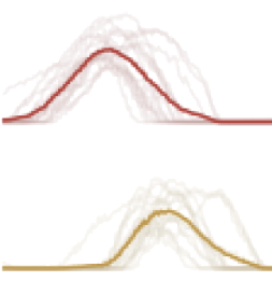
\includegraphics[width=\textwidth]{figures/curve_detector_radial_tuning.png}
\end{column}
\begin{column}{0.6\textwidth}
Rotating a stimulus smoothly transfers activation between orientation-selective detectors.
Together, they tile the full 360 degrees.
\end{column}
\end{columns}

\note{
\begin{itemize}
\item If we take dataset examples that cause a neuron to fire and rotate them, they gradually stop firing and the curve detector in the next orientation begins firing
\item This shows they detect rotated versions of the same thing
\item Together, they tile the full 360 degrees of potential orientations
\end{itemize}
}
\end{frame}

\begin{frame}{Argument 5: Feature Implementation \cite{olah2020}}
\begin{columns}[c]
\begin{column}{0.4\textwidth}
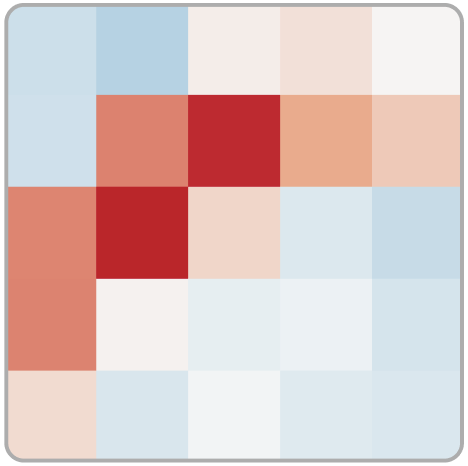
\includegraphics[width=\textwidth]{figures/curve_detector_weights.png}
\end{column}
\begin{column}{0.55\textwidth}
A curve detection algorithm can be read off the weights.
No evidence of a secondary cause of firing.
\end{column}
\end{columns}

\note{
\begin{itemize}
\item Circuit-based argument
\item By looking at the circuit constructing the curve detectors, we can read a curve detection algorithm off of the weights
\item We don't see anything suggestive of a second alternative cause of firing
\end{itemize}
}
\end{frame}

\begin{frame}{Argument 6: Feature Use \cite{olah2020}}
\begin{columns}[c]
\begin{column}{0.35\textwidth}
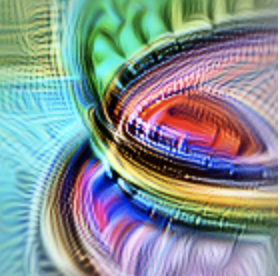
\includegraphics[width=\textwidth]{figures/curve_detector_use_in_circuits.png}
\end{column}
\begin{column}{0.6\textwidth}
Downstream clients are features that naturally involve curves: circles, spirals, 3d curvature.
\end{column}
\end{columns}

\note{
\begin{itemize}
\item Circuit-based argument
\item The downstream clients of curve detectors are features that naturally involve curves (circles, 3d curvature, spirals)
\item The curve detectors are used by these clients in the expected manner
\end{itemize}
}
\end{frame}

\begin{frame}{Argument 7: Handwritten Circuits \cite{olah2020}}
\begin{columns}[c]
\begin{column}{0.35\textwidth}
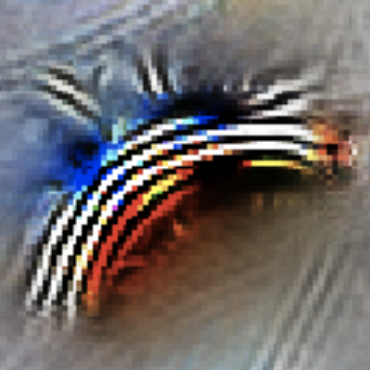
\includegraphics[width=\textwidth]{figures/arg_hand.png}
\end{column}
\begin{column}{0.6\textwidth}
We can do a cleanroom reimplementation, hand-setting all weights to reimplement curve detection.
These handwritten weights significantly mimic the original.
\end{column}
\end{columns}

\note{
\begin{itemize}
\item Circuit-based argument
\item Based on our understanding of how curve detectors are implemented, we can do a cleanroom reimplementation
\item Hand setting all weights to reimplement curve detection
\item These weights are an understandable curve detection algorithm, and significantly mimic the original curve detectors
\end{itemize}
}
\end{frame}

\begin{frame}{A Complex Feature: Cars in Superposition \cite{olah2020}}
\begin{center}
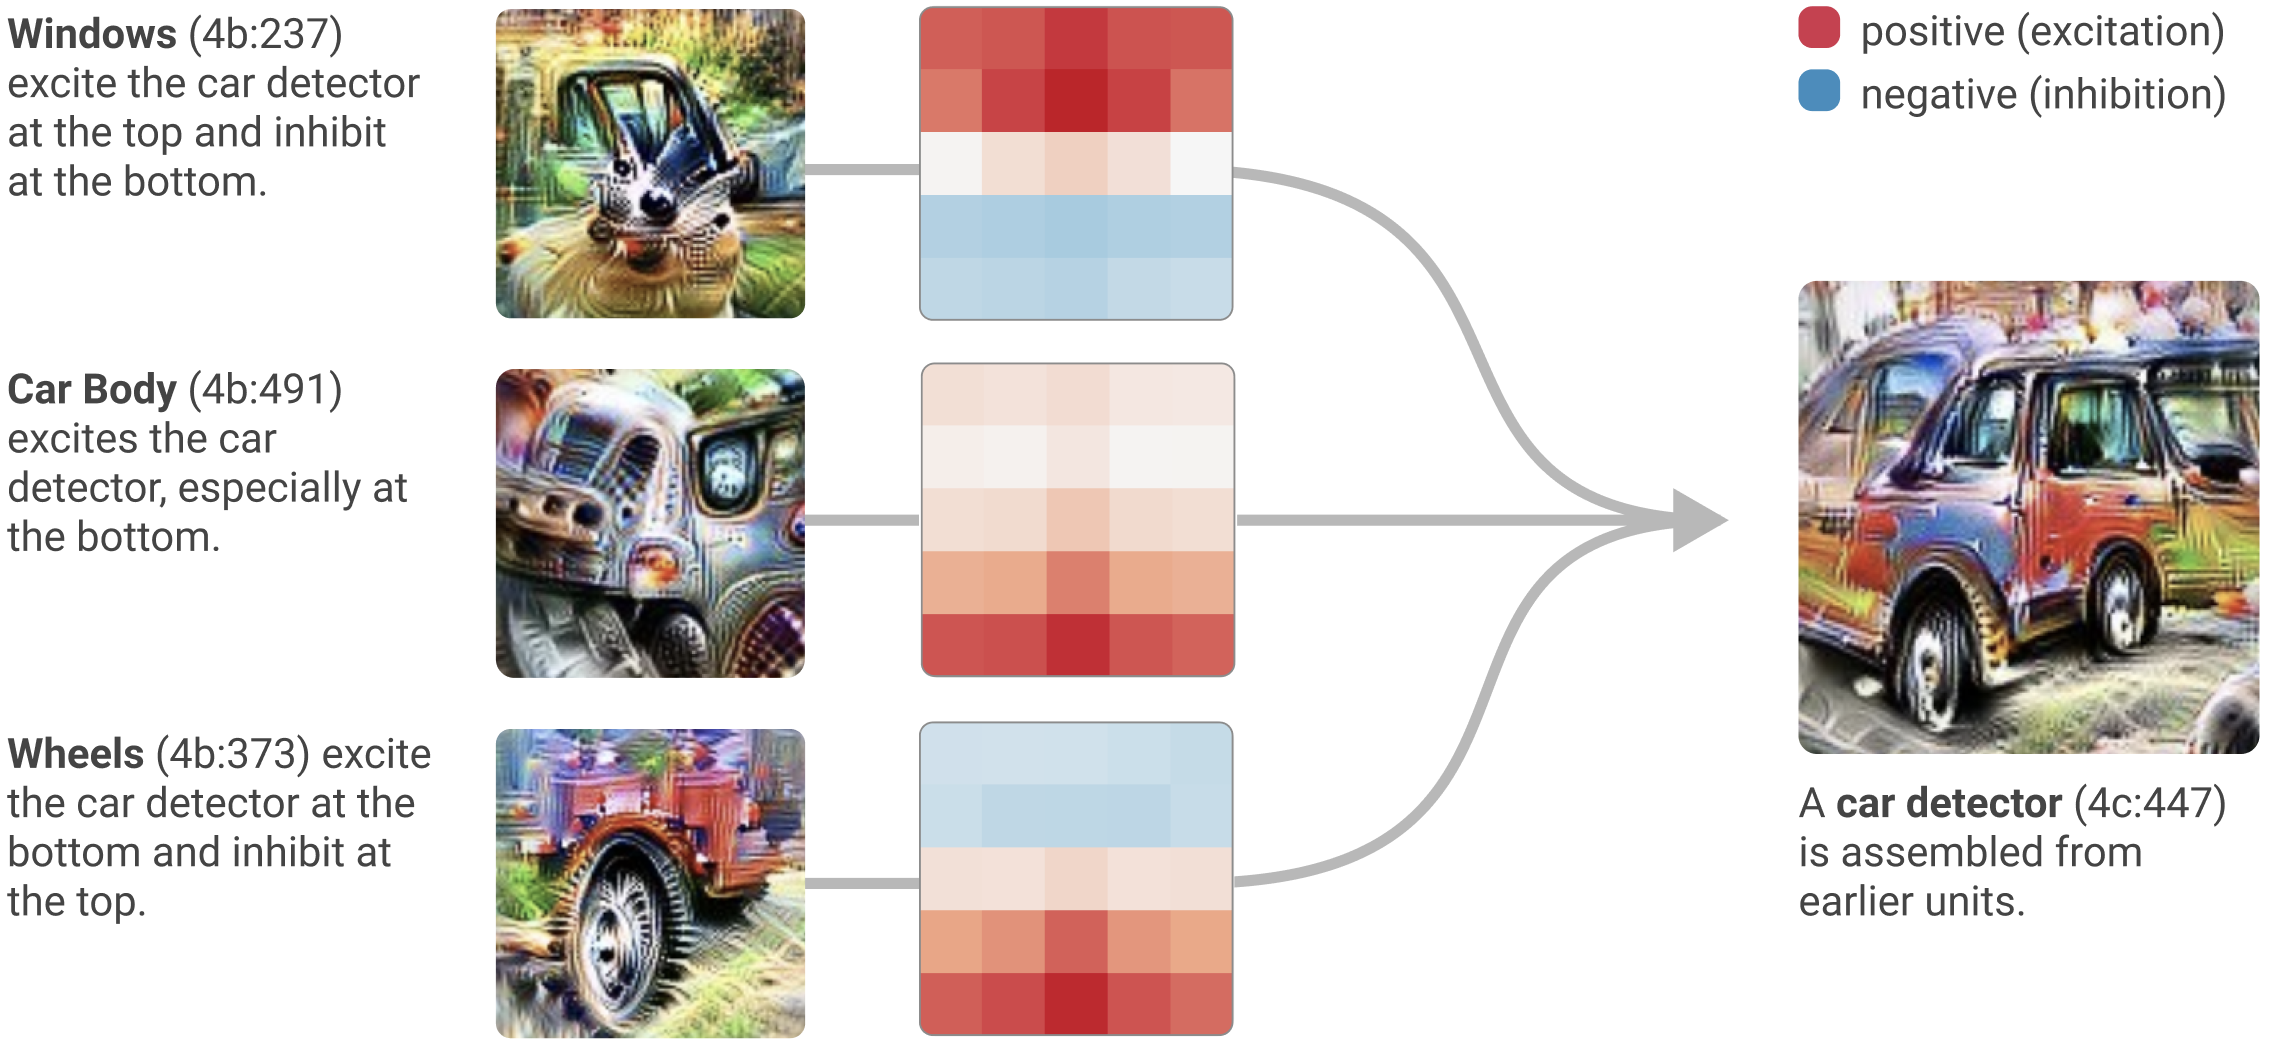
\includegraphics[width=0.85\textwidth,height=0.75\textheight,keepaspectratio]{figures/car_circuit.png}
\end{center}

\note{
\begin{itemize}
\item These methods also work to identify more complex structures
\item Note that these are still human-understandable
\item We can even understand the circuit here
\end{itemize}
}
\end{frame}

\begin{frame}{Universality in Image Models \cite{olah2020}}
\begin{columns}[t]
\begin{column}{0.48\textwidth}
\centering
{\large\textbf{Curve Detectors}}

\vspace{0.3em}
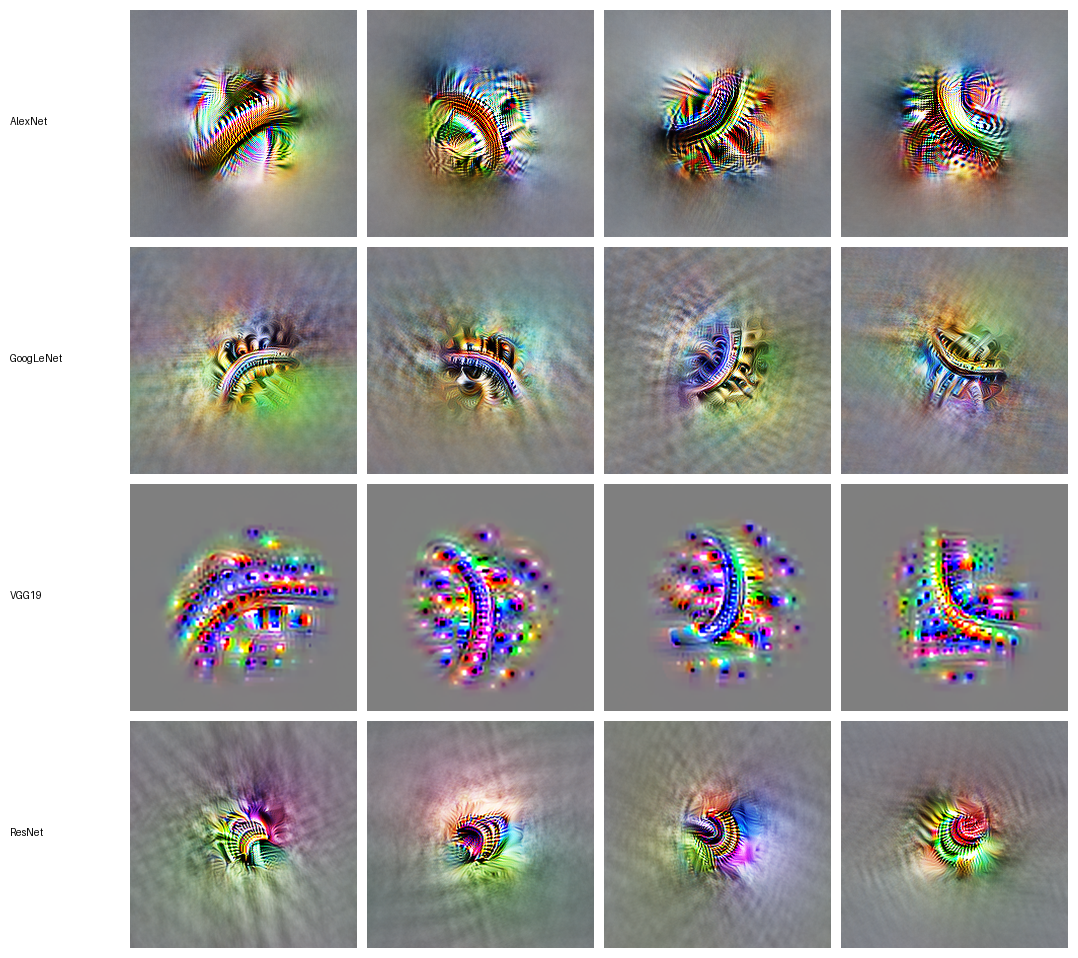
\includegraphics[width=\textwidth,height=0.65\textheight,keepaspectratio]{figures/universality_curves_full.png}
\end{column}
\begin{column}{0.48\textwidth}
\centering
{\large\textbf{High-Low Frequency Detectors}}

\vspace{0.3em}
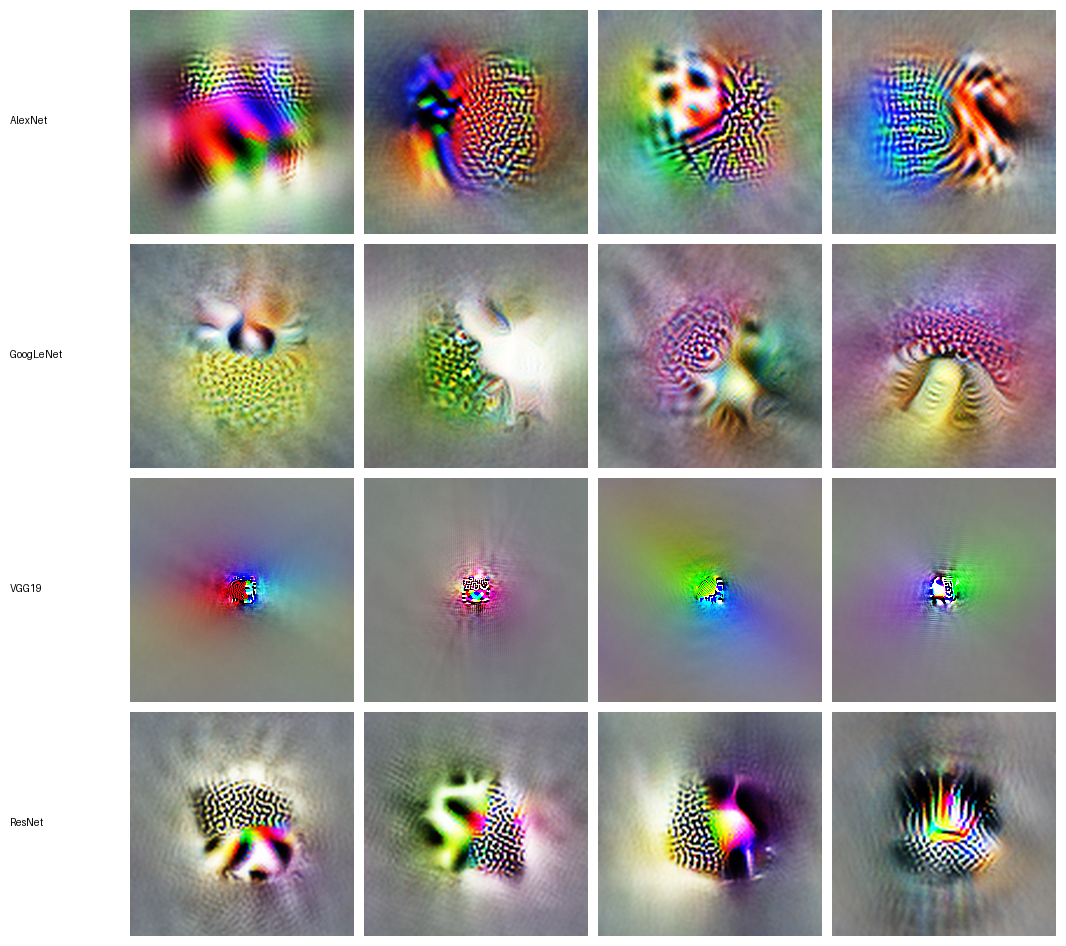
\includegraphics[width=\textwidth,height=0.65\textheight,keepaspectratio]{figures/universality_hilo_full.png}
\end{column}
\end{columns}
\vfill
{\small Rows: AlexNet, GoogLeNet, VGG19, ResNet}

\note{
\begin{itemize}
\item In image models, these features at least in early layers seem to be pretty universal
\item Curve detectors and high-low frequency detectors appear across AlexNet, GoogLeNet, VGG19, and ResNet
\item Later layers often correspond to human concepts, which speaks for their universality
\item But many channels do not seem to have easily understandable descriptions
\end{itemize}
}
\end{frame}

\begin{frame}{Polysemanticity \cite{olah2020}}
\begin{center}
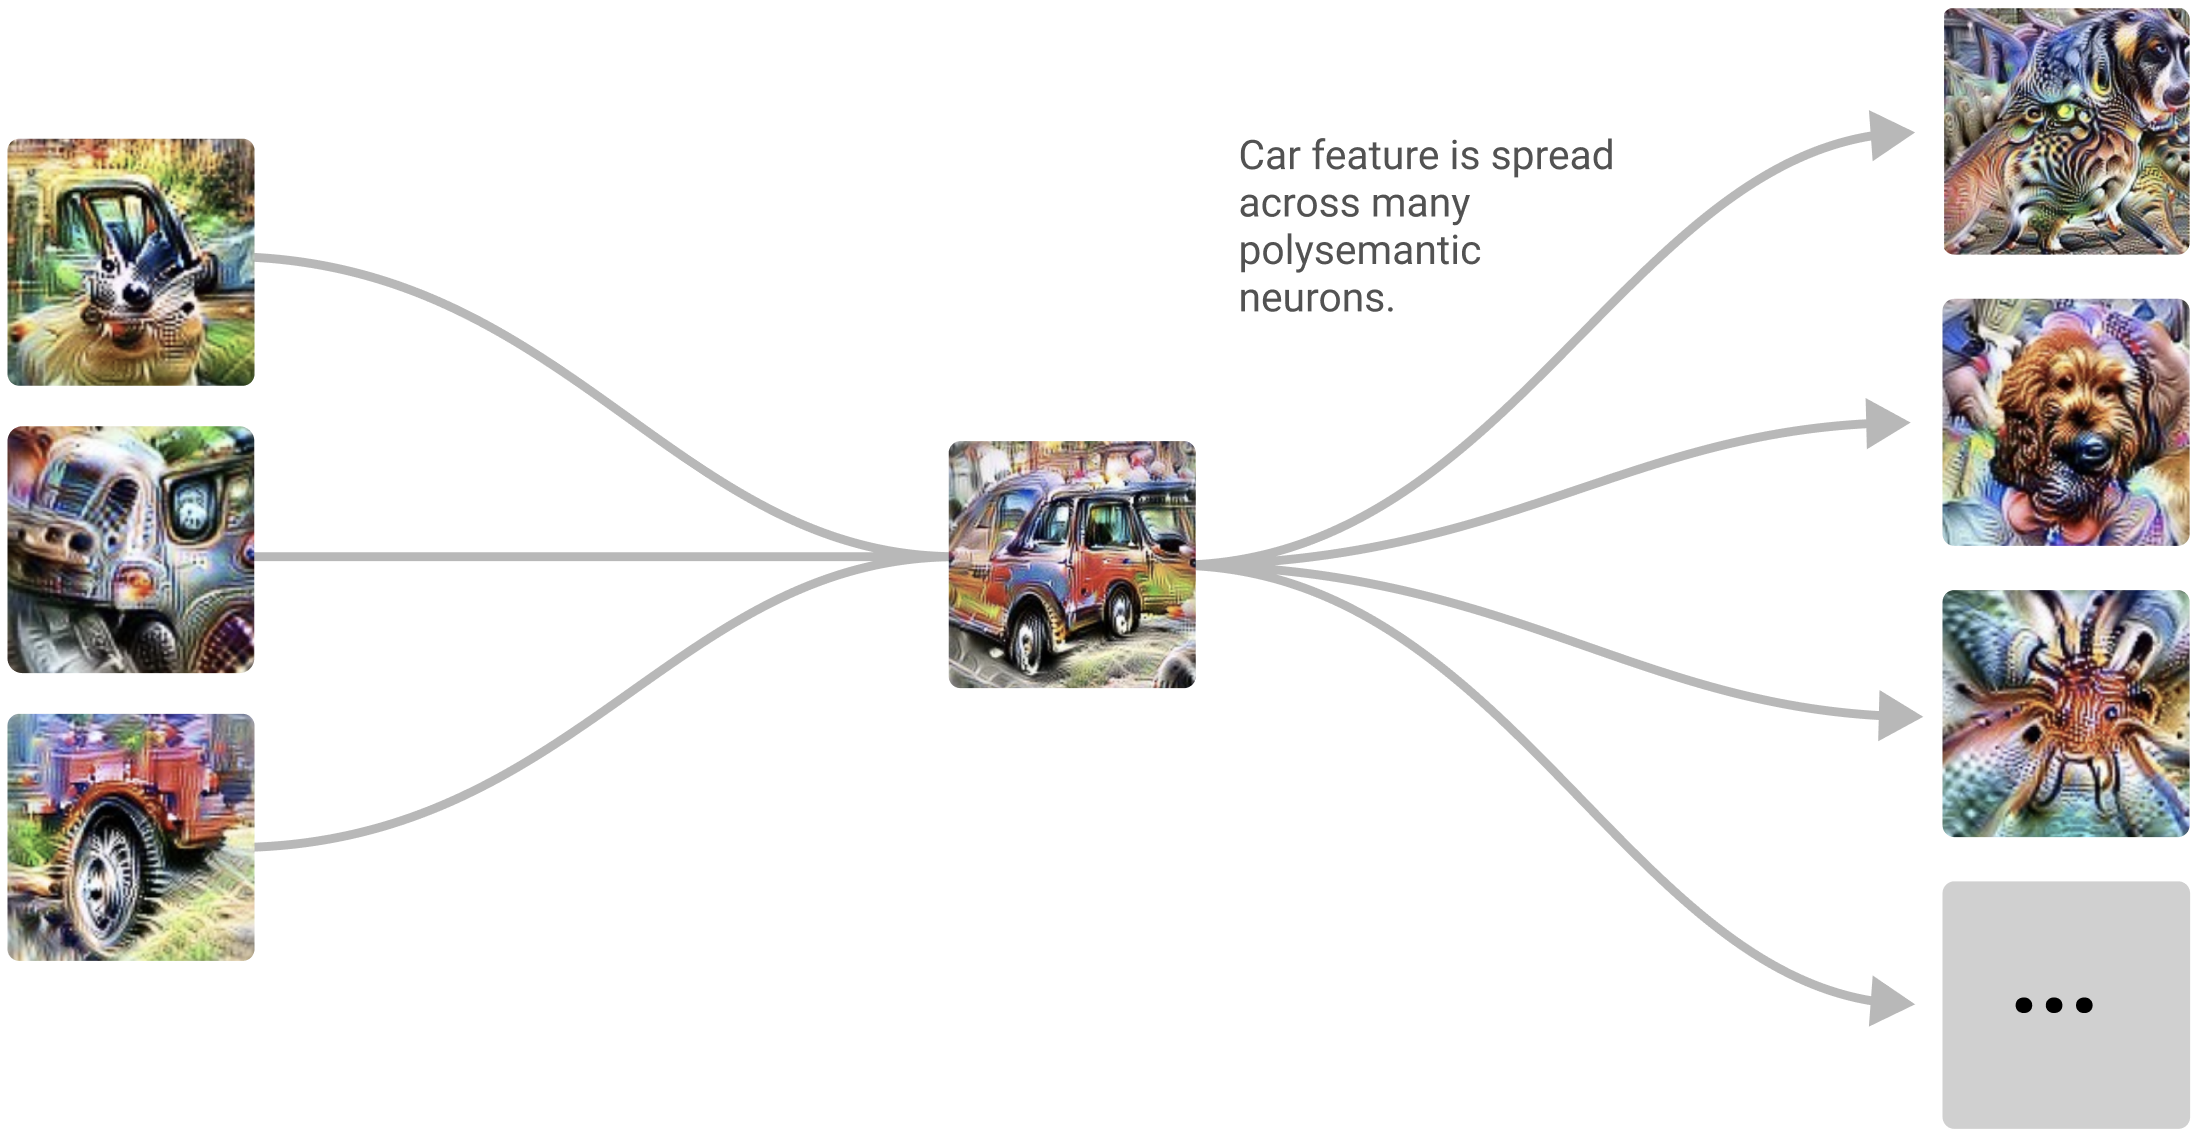
\includegraphics[width=0.85\textwidth,height=0.7\textheight,keepaspectratio]{figures/superposition.png}
\end{center}

\note{
\begin{itemize}
\item One problem, that we will discuss later, but is already visible in these models
\item Sometimes a feature is split up across different neurons, and multiple features share one neuron
\item Here we see that the car feature is assembled in one layer, but does not get its own neuron in a later layer
\item Its activations are split and added onto a bunch of other neurons that encode unrelated things
\item We can already see that this is necessary when we want to have more features than we have neurons
\end{itemize}
}
\end{frame}

\begin{frame}{If Universality Is True \cite{wentworth2020, chan2023}}
\begin{itemize}
\item What features are universal? Why?
\item Discussed in the Natural Abstractions discourse
\end{itemize}

\note{
\begin{itemize}
\item For curves this is obvious, but it is not clear how far this universality scales
\item Even if it does, it is not clear why those concepts in particular are universal
\item This might be pretty important: if we find a ``morally good'' feature in LLMs, do we expect it to behave the same as the human concept OOD in the limit of a super capable model?
\item Unclear, there are some theories here. AFAIK the work in this direction has stalled out the last years
\end{itemize}
}
\end{frame}
